\chapter{BioMotifInference.jl: Independent component analysis motif inference by nested sampling}
\chaptermark{BMI.jl: ICA motif inference by nested sampling}
\label{chap:BMI}
\section{Introduction}
While many methods to detect overrepresented motifs in nucleotide sequences, only one is a rigorously validated system of statistical inference that allows us to calculate the evidence for these motif models, given genomic observations: nested sampling \cite{Skilling2006}. Computational biologists almost immediately benefitted from Skilling's original publication, with the release of the Java-coded nMICA by Down et al. in 2005 \cite{Down2005}. Unfortunately, this code base is no longer being maintained. It is, moreover, desireable to take advantage of modern languages and programming techniques to improve the maintainability and productivity of important bioinformatic code. We therefore re-implemented Skilling's original algorithm, for use in inference of DNA motifs in Julia \cite{Bezanson2015}, as \path{BioMotifInference.jl}, hereafter \path{BMI.jl}.

In brief, \path{BMI.jl} is intended to estimate the evidence for \hyperref[ssec:ICA]{Independent Component Analysis} models of \hyperref[ssec:PWM]{Position Weight Matrix} (PWM) signals on \hyperref[ssec:HMM]{Hidden Markov Models} of genomic background noise (summarized in \autoref{fig:BMIschematic}), and to estimate the \hyperref[ssec:MLE]{maximum a priori} parameters of detected signals. This allows the user to perform Bayesian model selection and comparison for generative hypotheses about genomic sequences of interest. The ICA approach is discussed in more detail in the relevant sections of \autoref{chap:theoryA}.

\begin{figure}
    \makebox[\textwidth][c]{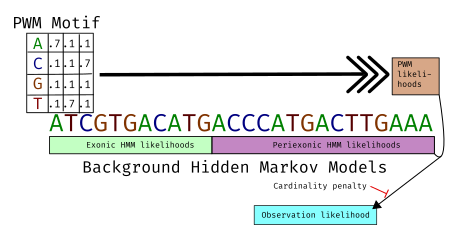
\includegraphics[width=.8\textwidth]{IPMlh.png}}    
    \caption{{\bf Schematic representation of BioMotifInference likelihood algorithm.}}
    \label{fig:BMIschematic}
\end{figure}

\section{Implementation of the nested sampling algorithm}

Skilling's nested sampling algorithm is accompanied with an almost-certain guaranteed to converge an ensemble of models on the global optimum likelihood in the parameter space \cite{Skilling2006}. An important assumption underpinning this guarantee is that the sampling density (in effect, the size of the ensemble) be high enough that widely separated modes are populated by at least one model each. Although early suggestions for the generation of new models within the ensemble were generally to decorrelate existing models by diffusional \hyperref[ssec:MonteCarlo]{Monte Carlo} permutation, later work generally acknowledges that this can be highly inefficient \cite{Skilling2012}, particularly in large parameter spaces with many modes, of which the sequence parameter spaces explored in \autoref{chap:rys} are good examples. A number of ways of addressing this problem have arisen in the cosmology and physics literature. These include improved sampling methods, such as sampling within an ellipsoidal hypersphere encompassing the positions of the ensemble models within the parameter space \cite{Feroz2008,Feroz2009} or Galiliean Monte Carlo (GMC) \cite{Skilling2012}, as well as methods of increasing computational efficiency, such as dynamic adjustment of ensemble size \cite{Higson2019}. 

Generally speaking, these methods are not good candidates for \path{BMI.jl} because the PWM representation of sequence signal in the ICA PWM model (IPM) is makes ordinary parameter space representation much less efficient. This is for at least four reasons:

\begin{enumerate}
    \item\label{identicalmodels} Identical IPMs may be expressed with their vector of PWM sources (or "channels") in different orders, so the parameter space becomes increasingly degenerate with higher numbers of sources.
    \item Closely equivalent repetitive signals can be represented by PWMs on opposite ends of the parameter space (e.g. ATAT vs TATA), reducing the efficiency of ellipsoidal sampling methods and introducing a further degeneracy.
    \item If model likelihoods are being calculated on the reverse strand of observations, sources on opposite ends of the parameter space (ie. reverse complements) can also represent closely equivalent signals, introducing another source of degeneracy.
    \item IPM sources may be of different lengths. Even if we can relate sources in different models to one another by some consistent distance rule, it is unclear how one would decide which dimensions of longer sources to project the parameters of shorter ones into. BioMotifInference does maintain an index for each source against its prior, but this is no guarantee that sources remain in some way "aligned". Rather, some type of alignment would have to be done, probably significantly increasing computational cost\footnote{Probably some combination of dimensional analysis and fast alignment algorithms could make some headway here.}.
\end{enumerate}

While it is possible to perform Markov Chain Monte Carlo in a manner that allows jumps between differently-dimensioned models in detailed balance, this applies only to diffeomorphic transformations \cite{Hastie2012}. PWM models are not merely matrices of unrelated parameters, but are an ordered sequence of 4-parameter discrete Categorical distributions. If the addition or removal of a discrete, indexed set of 4 parameters to an existing vector of such sets can be made reversible in this manner, the proof is beyond the scope of the present work. Therefore, BioMotifInference (BMI) is not likely in strict detailed balance over a well behaved parameter space, given its default permute functions and configuration. Permute functions are designed around pragmatic concerns associated with the flow of model information in the IPM ensemble, and are tuned for computational efficiency in producing permuted models that are more likely than the starting model. The justification for this is simply feasibility; doing this allows an ensemble to be converged on larger samples from genome-scale datasets. Because of the flexible nature of the sampler, the user may easily specify \path{BMI.jl}-compatible permute functions, should better ones for their application be apparent to them.

It should be noted that these considerations do not entirely preclude the operation of the \path{BMI.jl} in detailed balance over the prior. This can be achieved by the user specifying a single length for the PWM sources (rather than a range of permissible lengths), and using a permutation routine consisting solely of the functions \path{random_decorrelate} and \path{reinit_src}, along with any user-defined functions coded with the detailed balance stricture in mind. Operation in this fashion may improve the accuracy of both evidence estimates and the sources found in the maximum a posteriori (MAP) sample defined by the converged ensemble. That said, unless the supplied prior is unusually good, this mode of operation is only well suited to very small observation sets, on the order of kilobases. With uninformative priors and good background models, the vast majority of sources sampled from the prior will receive significant likelihood penalties relative to the background model alone. Performing nested sampling on such an ensemble by diffusional techniques, in good detailed balance, will usually fail to produce models more likely than the background model within any reasonable compute budget, and will generally never converge. The feasibility constraint thus justifies the use of bespoke sampling routines for genome-scale datasets.

Like its predecessor \path{nMICA}, \path{BMI.jl} samples new models by applying one of a collection of permutation functions to an existing model. Additionally, although \path{BMI.jl} is supplied prior distributions on IPM parameters from which the initial ensemble is sampled, there is no way provided to calculate a posterior from the models generated by the nested sampling process, largely because of the identical source issue, \ref{identicalmodels}. The primary outputs of interest are the estimation of the Bayesian evidence ratios between models (the absolute values of evidence are unlikely to be accurate)\footnote{It is not clear that evidence ratios solve the accuracy problem [Kevin Knuth, personal correspondence, 2021]. The best that can be said about this is that a larger ratio in favour of some model is more likely to reflect an actual preponderence of evidence in its favour. For this reason, the MAP sample may be the most informative part of BMI output.}, as well as the models in the final ensemble (which constitute samples from the MAP mode or modes).

Because the more conventional methods to address the inefficiency of nested sampling by Monte Carlo used in cosmological models described above are unavailable, \path{BMI.jl} uses an ad hoc method of adjusting the mixture of permute patterns that are applied to models. The basic permute logic (encoded by \path{Permute_Instruct} arguments to the \path{permute_IPM} function) is as follows:

\begin{enumerate}
    \item\label{selectmodel} Select a random  model from the ensemble.
    \item\label{applyfunc} Apply a randomly selected permutation function from the instruction's function list according to the probability weights given to the functions by the instruction's weight vector.
    \item Repeat \ref{applyfunc} until a model more likely than the ensemble contour, given observations, is found, or the instruction's \path{func_limit} is reached.
    \item If the \path{func_limit} is reached without a new model being found, return to \ref{selectmodel} and repeat \ref{applyfunc} until a model more likely than the ensemble's contour is found, or until the instruction's \path{model_limit} is reached.
\end{enumerate}

\section{Usage notes}
\subsection{Preparation of observation set}
\path{BMI.jl} relies on \path{BioBackgroundModels.jl} both for selecting appropriate background models for motif inference, as well as to code observations and prepare an appropriate matrix of background scores. The selection of background models is covered in \autoref{chap:BBM}. The coding of observations requires the construction of a \path{DataFrame} containing a column of type \path{Vector{LongSequence{DNAAlphabet{2}}}}, the unambiguous DNA alphabet of \path{BioSequences.jl}. This is accomplished as follows:

\begin{minted}[breaklines,
    mathescape,
    linenos,
    numbersep=5pt,
    frame=lines,
    framesep=2mm]{julia}
    using BioBackgroundModels, DataFrames, Serialization
    obspath=/path/to/observations_dataframe
    obs_df=deserialize(obspath)
    coded_obs=observation_setup(obs, order=0, symbol=:seq)\end{minted}

Note that \path{observation_setup} must be supplied an \path{order} keyword argument of 0; while \path{BMI.jl} supports background HMMs of any order, signal motifs are 0\textsuperscript{th} order. If the name of the sequence column of the observations \path{DataFrame} differs from ``Seq'', a symbol specifying the column name should be passed as the \path{symbol} keyword argument.

To construct the background matrix, the observations must be masked by partition, and the positional likelihoods of the sequences calculated:

\begin{minted}[breaklines,
    mathescape,
    linenos,
    numbersep=5pt,
    frame=lines,
    framesep=2mm]{julia}
    BioBackgroundModels.add_partition_masks!(obs_df, genome_gff_path, 500, (:chr,:seq,:start))

    BHMM_dict = Dict{String,BHMM}()
    reports_folder=deserialize(/path/to/BBM_Reports_Folder)
    for (partition, folder) in reports_folder
        BHMM_dict[partition]=folder.partition_report.best_model[2]
    end

    background_scores=BGHMM_likelihood_calc(obs_df, BHMM_dict, symbol=:seq)\end{minted}

\path{add_partition_masks!} adds a mask column to the observations \path{DataFrame}, which is used by \path{BGHMM_likelihood_calc} to determine the correct background model to use for any given base in the observations sequence. It requires a path to a valid GFF3 annotation file for the genome. In order for the observations to be masked correctly, a tuple of column names containing the scaffold ID the observation is found on\footnote{It must be ensured that this ID corresponds to the one used by the GFF3}, the sequence on the positive strand, and the start position of the sequence on the scaffold.

The calculation of background scores requires a \path{Dict} of \path{BBM.jl} background models keyed by the partition ID. In the example, this is constructed programmatically from a \path{Report_Folder}; see \autoref{chap:BBM} for the generation of these reports.

\subsection{\protect\path{IPM_Ensemble} assembly}
Once the coded observation set and the matrix of background scores are prepared, an \path{IPM_Ensemble} may be initialised by sampling from a prior. Priors must first be assembled. This process is executed as follows:

\begin{minted}[breaklines,
    mathescape,
    linenos,
    numbersep=5pt,
    frame=lines,
    framesep=2mm]{julia}
    num_sources=5
    source_length_range=3:10
    uninformative_mixing_prior=.1
    source_prior = BioMotifInference.assemble_source_priors(num_sources, Vector{Matrix{Float64}}())
    mix_prior = (falses(0,0), uninformative_mixing_prior)

    e = BioMotifInference.IPM_Ensemble(worker_pool, "/path/to/ensemble/", ensemble_size, source_prior, (falses(0,0), mixing_prior), background_scores, coded_obs, source_length_range, posterior_switch=true)
\end{minted}

Here, an uninformative prior is assembled for 5 sources. If we wanted to supply some PWM samples create informative Dirichlet priors from, these would be supplied in the vector of matrices passed as the second positional argument to \path{assemble_source_priors}. Informative priors are produced by multiplying the PWM values by a fixed weight, which may be passed as the keyword argument \path{wt}.

An uninformative prior is supplied for the mixing matrix. The prior tuple consists of an empty \path{BitMatrix}; if an informative prior is desired, the appropriate \path{BitMatrix} for the informative sources is passed instead. Sources for which no informative prior is supplied have their mix vectors sampled from a fractional floating point success rate prior. Here, the \path{uninformative_mixing_prior} is .1, meaning that an average of 10\% of observations will be initialized with each source.

Sampling and likelihood calculations may be performed in parallel by submitting a valid integer vector worker pool as the first positional argument ot \path{IPM_Ensemble}, or conducted by the master process if this is omitted. Passing \path{true} for the keyword argument \path{posterior_switch} will ensure that the least likely models, discarded from the ensemble during the sampling procedure, are collected as samples from the posterior distribution. This is \path{false} by default, as no rigorous method for estimating posterior distributions is available.

\subsection{Permute routine setup}
\label{ssec:adhoc}
In order to converge an assembled \path{IPM_Ensemble} by nested sampling, it is necessary to provide an initial \path{Permute_Instruct}, which determines sampler behaviour, and is tuned by the \path{Permute_Tuner} to prioritize permute functions which currently produce the largest positive particle displacements over the likelihood surface in parameter space, per computational time. Some application-specific tweaking is usually necessary. Depending on how the computation is to be parallelized, the weights assigned ot network-intensive functions by the tuner, in particular, may benefit from being clamped. In order to convey how to set up an initial \path{Permute_Instruct} successfully, notes regarding the operation of the stock permute functions on \path{ICA_PWM_Model}s (IPMs) is summarized below. In this discussion, ``premature homogenisation'' refers to the loss of sampling density in relevant parts of the posterior, so that the ensemble particles are trapped in some local optimum.

\begin{itemize}
    \item \path{permute_source}: randomly permutes a single source in the IPM by altering the PWM weights or changing the length of the source. Distributions for the frequency and size of these permutations may be supplied. If the size of the perturbations is small, and the frequency of length changes is set to 0., this function is useful for finding sources that are slightly more probable than the current ones.
    \item \path{permute_mix}: flip a random number of mix matrix positions. Retains flips that make observations more probable. If the range of flip moves is kept small, this is a useful function for ``polishing'' the mix matrix, particularly of models with highly probable sources. Effective throughout the sampling process.
    \item \path{perm_src_fit_mix}: as \path{permute_source}, but the permuted source is supplied with a new mix vector which mixes the source solely into observations that it makes more probable. Efficient and effective throughout the sampling process.
    \item \path{fit_mix}: checks each source against each observation, mixes only those sources that make the observation more probable in isolation. By far the most important permute during the early sampling process, since it can quickly move improbable models sampled from uninformative priors into the portion of the parameter space with likelihoods greater than the background model. In effect, this allows the extraction of maximum information about the data from the initial sampling process, which typically produces many widely divergent sources. This prevents premature homogenisation of the ensemble after extensive sampling below the background model likelihood, and subsequent distortions of evidence and maximum a posteriori parameter estimates.
    \item \path{random_decorrelate}: perform the operations of \path{permute_source} and \path{permute_mix} on the same model. This is an inefficient permute in general, but it is useful for introducing new sources during the early part of a sampling run, in particular, working to prevent premature homogenisation.
    \item \path{shuffle_sources}: copy the source PWM from another model in the ensemble, leaving the original mix matrix. This can be an effective permute early in the sampling process. It is network intensive.
    \item \path{accumulate_mix}: randomly select a source from the model to be permuted. From another model in the ensemble, select the source which is most similar to the one selected in the original model. Add the two mixvectors together, such that the original source is now mixed in to any observations in the second model that had the similar source. This is an extremely effective permute when the ensemble begins to have many similar sources in different models, and often is the best way to produce models more likely than those produced by \path{fit_mix}. Network intensive. This is sometimes the last permute that can find model parameterisations more probable than those in a well-converged ensemble. Network intensive.
    \item \path{distance_merge}: Randomly select a source from the model to be permuted. From another model in the ensemble, select the most dissimilar source, and overwrite the selected source in the original model with the PWM and mixvector from this dissimilar source. This can be an effective permute throughout the sampling process. It tends to encourage the propagation of likely sources through the ensemble. Network intensive.
    \item \path{similarity_merge}: As \path{distance_merge}, except the most similar source is selected, and the original mixvector is retained. This tends to be less efficent than \path{distance_merge}, but can find new models throughout the sampling process. Network intensive.
    \item \path{reinit_src}: Resample a random source in the model to be permuted from the prior. This is a very inefficient permute, mostly useful in the early part of the sampling process to reintroduce sources from undersampled parts of the prior.
    \item \path{erode_model}: Trim a source's PWM in the model to be permuted to only those positions whose weight vectors express information above a threshold. This has the effect of generating high-likelihood short sources from longer ones with stretches of uninformative postions. It is mostly useful in the early part of the sampling process.
    \item \path{info_fill}: For a random source in the permute model, find the least informative PWM position, and set the probability of the most informative base to 1. This function assists in preventing premature homogenisation by rapidly increasing the likelihood of sources that are well-supported by observations but are unlikely to achieve appropriate high PWM weights by random permutation alone.
\end{itemize}

A \path{Permute_Instruct} requires a vector of the functions to be used in the permutation routine, a corresponding vector of their initial weights (ie. the frequency with which they will be called), a limit on the number of models to permute before the worker abandons sampling, and a limit on the number of functions to apply to any given model before selecting a new one to attempt permuting. The annotated example provided below also passes, as keyword arguments, vectors of minimum and maximum weights (\path{min_clmps} and \path{max_clmps}), as well as a vector of keyword arguments for the vector of functions (\path{args}).

\begin{minted}[breaklines,
    mathescape,
    linenos,
    numbersep=5pt,
    frame=lines,
    framesep=2mm]{julia}
    funcvec=full_perm_funcvec #exported by BMI.jl
    models_to_permute=10000
    func_limit=25
    
    #add two ``polishing functions'' to the function vector
    push!(funcvec, BioMotifInference.perm_src_fit_mix) 
    push!(funcvec, BioMotifInference.random_decorrelate)
    
    #all functions will receive a minimum of 1 in 100 function calls
    min_clamps=fill(.01,length(funcvec))

    #give some important functions a minimum of 10 in 100 function calls
    min_clamps[2:3].=.1 #perm_src_fit_mix & permute_mix
    min_clamps[8]=.1 #difference_merge

    #no function will receive more than 50 in 100 function calls
    max_clamps=fill(.5,length(funcvec))

    #prevent network intensive functions from swamping the cluster
    max_clamps[6:7].=.15 #shuffle_source and accumulate_mix
    max_clamps[9]=.15 #similarity_merge
    
    #evenly distributed initial weights
    initial_weights= ones(length(funcvec))./length(funcvec)
    
    #empty arguments vectors for all arguments in the funcvec
    args=[Vector{Tuple{Symbol,Any}}() for i in 1:length(funcvec)]
    
    #add arguments for the ``polishing functions''
    args[end-1]=[(:weight_shift_freq,0.),(:length_change_freq,1.),(:length_perm_range,1:1)]
    args[end]=[(:iterates,50),(:source_permute_freq,.3),(:mix_move_range,1:10)]
    
    #instantiate the Permute_Instruct
    instruct = Permute_Instruct(funcvec, initial_weights, models_to_permute, func_limit;min_clmps=min_clamps, max_clmps=max_clamps, args=args)
\end{minted}

\subsection{Nested sampling of \protect\path{IPM_Ensemble}s}

When all of the above tasks are complete, the \path{IPM_Ensemble} may be converged by nested sampling using the specified permutation routine. This can be performed in parallel; any number of permutation workers may be used. However, because the master process is responsible for disk access, many such workers performing permutation functions which frequently require the deserialization of other models in the ensemble (those noted as ``network intensive'' above) will rapidly reduce the computational efficiency of the cluster. This can be mitigated by clamping network intensive permute functions to a lower frequency of total function calls.

\path{BMI.jl} is supplied with a display system similar to, but less customisable than \path{GMC_NS.jl}. An example of display setup and nested sampling execution is presented below:

\begin{minted}[breaklines,
    mathescape,
    linenos,
    numbersep=5pt,
    frame=lines,
    framesep=2mm]{julia}

display_rotation=[true,10,1,[[:tuning_disp,:lh_disp,:src_disp],[:conv_plot,:liwi_disp,:ens_disp]]]

logZ = converge_ensemble!(e, instruct, worker_pool, backup=(true,25), tuning_disp=true, lh_disp=true, src_disp=true, disp_rotate_inst=display_rotation)
\end{minted}

\section{Test of model comparison logic with spiked motifs}
Because the proper functioning of \path{BMI.jl} is difficult to verify, we constructed a test problem to ensure that the package can, in principle, be used to distinguish between synthetic observation sets spiked with two different sets of motifs, representing separate causal processes. This is done by generating two sets of 500 synthetic observations of 100-200 bases in length, and spiking them with different periodic, repetitive signals, as well as aperiodic, randomly occuring transcription factor motifs (a TATA box and a CAAT box). Ensembles of 250 \hyperref[ssec:ICA]{ICA} models with two PWM sources between 3 and 12 bases in length are assembled, one for each of the two separate observations sets, and one to model the combined set. Code to estimate the evidence for these ensembles in available in \autoref{ssec:spike_recovery}. Execution of this code gives a logZR of 110.87 ± 0.88 in favour of the separate models. While the uncertainty on this value is unreliable, the result suggests that the algorithm is capable of distinguishing properly between observations sets generated by separate causal processes on similar backgrounds.

\section{Future Directions}
The prospects for \path{BMI.jl} are limited by the difficulty in ensuring the sampling routines are in detailed balance. It is possible that this could be resolved. One possibility might be to implement a form of \hyperref[ssec:GMC]{Galilean Monte Carlo} by giving models a three-dimensional coordinate for each base pair in each source channel (fixing the number of bases per source). This coordinate would encode the location of the model within a tetrahedral probability 3-simplex (this is discussed further in \autoref{ssec:PWM}, about Position Weight Motif models). The boolean mixing matrix could, perhaps, also be subject to GMC, if at each mix matrix position the model had either positive, negative, or zero velocity.

This solution would not directly solve the degeneracy issues mentioned above, but it may allow for more accuracy in evidence estimation. The dimensionality implied by this parameterisation is nonetheless high. The models used in \autoref{chap:rys} contain eight PWM sources of 3-10 bases in length. If we fix the PWM length at 5 bases, there are 120 parameters for the PWM sources alone. Practically speaking, this kind of solution is likely to be best employed where only a few, short, repetitive sequences are of interest.

One way to address the error associated with ad hoc sampling routines might be to construct small toy problems with known model evidence; different sampling routines could be tested on these to perform a stretch test, measuring actual sampler performance against the theoretical distribution of compressive steps \cite{Buchner2016}. If this is possible, the effects of the \path{BMI.jl} tuning regimen could be characterised and error minimised.